%---------------------------------
%---------------------------------
\chapter{Biologie der Wirbeltiere}
\label{chapter:biology}
% eventuell als Abschnitt in "`Grundlagen"'?

\begin{center}
 \begin{minipage}{12cm}
  \emph{"`Nichts anderes in der Natur hat eine herrlichere Struktur als der Körper der Wirbeltiere."'}
 
  --- "`Vergleichende und funktionelle Anatomie der Wirbeltiere"' \cite[S.\ 1]{Vergleichende_Anatomie}
 \end{minipage}
\end{center}

Dieses Kapitel soll einen Überblick über die biologische Beschaffenheit der Wirbeltiere geben. Da dies keine biologische Arbeit ist, werden nur diejenigen Merkmale und Eigenschaften weiter ausgeführt, die im Folgenden zum Verständnis nötig sind.

% Definition
Wirbeltiere, oder auch Vertebrata, sind Tiere mit einer skelettartigen Schädelkapsel, einem Cranium. Deshalb werden sie auch Schädeltiere oder Craniota genannt.\\
Auf den ersten Blick ist diese Definition etwas überraschend, da als  Haupteigenschaft nicht die Wirbelsäule, sondern der Schädel genannt wird. Das liegt daran, dass zu den Wirbeltieren auch einige Tiere gezählt werden, die gar keine Wirbelsäule sondern "`nur"' eine Chorda dorsalis besitzen. Die Chorda dorsalis besteht aus weichem Gewebe, nicht aus Knochen. Sie ist das Achsenskelett der Chordatiere, einem Tierstamm, zu dem auch die Wirbeltiere gehören. \cite[S.\ 27 f.]{Vergleichende_Anatomie}\\
Hier in dieser Arbeit soll es aber nur um Wirbeltiere mit Wirbelsäule gehen.

% 5 Klassen
Es gibt fünf große Gruppen von Wirbeltieren. Die historisch ersten Wirbeltiere sind die Fische. Danach entwickelten sich die Tetrapoden, Wirbeltiere mit vier Gliedmaßen, zu denen alle anderen Gruppen gehören. Zunächst entstanden die Amphibien, die noch nicht vollkommen terrestrisch leben. Daraus entwickelten sich die Reptilien, die erste Klasse der Wirbeltiere, die alle Strukturen besitzt um vollkommen an Land zu leben. (Es gibt aber auch Reptilien die trotzdem wieder im Wasser leben.) Außerdem gibt es noch die Vögel, die sich auf das Fliegen spezialisiert haben, und die Säugetiere, die ihre Jungen säugen. \cite[Kapitel 4]{Vergleichende_Anatomie}

Auch der Mensch ist ein Säugetier und besitzt eine Wirbelsäule. Da sich Wirbeltiere, vor allem in ihrem Skelett, sehr ähneln, lassen sich viele der im folgenden Abschnitt aufgeführten Eigenschaften des Skeletts, vermutlich leicht "`am eigenen Leib"' nachvollziehen.


\newpage
%------------------------------------
\section{Das Skelett}
\label{biology_skeleton}

\vspace{0.5cm}
\begin{center}
 \begin{minipage}{12cm}
  \emph{"`Das innere, gelenkige Skelettsystem der Vertebraten ist einzigartig im Tierreich. Es ist das wichtigste aller Organsysteme für das Studium der Wirbeltiermorphologie."'}
  --- \cite[S.\ 131]{Vergleichende_Anatomie}
 \end{minipage}
\end{center}


Wirbeltiere haben ein inneres Skelett und ihr Körper ist bilateralsymmetrisch \cite[S.\ 27]{Vergleichende_Anatomie}. Das bedeutet, dass ihre linke Körperseite symmetrisch zur rechten ist. 

\paragraph{Wirbelsäule}
Aufbau und Form der Wirbelsäule hängen von der Lebensweise des entsprechenden Wirbeltiers ab. Ein wesentlicher Einflussfaktor sind die Kräfte, die auf die Wirbelsäule wirken. 
Bei Fischen muss die Wirbelsäule dem Druck der starken Axialmuskeln, die seitlich am Körper entlang führen, entgegenwirken.
Bei Tetrapoden sind diese Axialmuskeln zurückgebildet, dafür muss die Wirbelsäule aber der Schwerkraft widerstehen.
Und bei Vögeln ist die Wirbelsäule speziell an den Flug angepasst und deshalb \ua besonders leicht. \cite[\mbox{Abschnitt 9.2}, S.\ 168 ff.]{Vergleichende_Anatomie}

% Wirbelanzahl
Auch die Anzahl der Wirbel unterscheidet sich teilweise erheblich. 
Die Halswirbelsäule ist \zb bei den Fischen noch gar nicht herausgebildet. Amphibien haben einen Wirbel, der für die Beweglichkeit des Kopfes zuständig ist. Bei Reptilien ist die Halsregion meist schon stärker abgesetzt. Säugetiere haben, bis auf wenige Ausnahmen, genau $7$ Halswirbel, egal wie lang der Hals ist. Vögel haben die meisten Halswirbel, nämlich $10$ bis maximal $31$ beim Trauerschwan \cite{WikipediaVogelskelett}, meistens aber zwischen $15$ und $20$. \cite[Abschnitt 9.2]{Vergleichende_Anatomie}

Ebenso unterscheidet sich die Anzahl der Wirbel in anderen Teilen der Wirbelsäule. Teilweise sind Wirbel sogar miteinander zu einem größeren Knochen verwachsen. Betrachtet man nur die Gruppe der Säugetiere, so kommt man auf etwa $12$ bis $14$ Brustwirbel, $5$ bis $7$ Lendenwirbel, $3$ bis $5$ Kreuzwirbel und $4$ bis $22$ Schwanzwirbel \cite{AnatomieKuenstler}.

% Wirbelform
Auch die Form der einzelnen Wirbel unterscheidet sich sowohl zwischen den verschiedenen Tieren als auch entlang der Wirbelsäule einer einzelnen Art \cite[Abschnitt 9.1 und \mbox{Abbildung 9.2}]{Vergleichende_Anatomie}. 
Um diese Vielfalt zu abstrahieren wird hier mit Platzhaltern gearbeitet, die für alle Arten von Wirbeln stehen. Falls später eine genauere Unterscheidung nötig sein sollte, können diese leicht spezialisiert werden.

\paragraph{Extremitäten}
Die Extremitäten der Tetrapoden sind nach einem "`Grundbauplan"' aufgebaut (siehe Abbildung \ref{extremities}a). Dieser wird jedoch vielfach abgewandelt. Einige Beispiele sind in Abbildung \ref{extremities}b zu sehen. \cite[S.\ 487]{AllgemeineZoologie}\\
Bei Fischen haben die Extremitäten keine Verbindung zur Wirbelsäule. Erst Amphibien bilden Schulter- und Beckengürtel aus, da sie zur Fortbewegung an Land nötig sind. \cite[Abschnitt 9.2.3]{Vergleichende_Anatomie}
Der Einfachheit halber wird hier aber nicht weiter beachtet ob eine Verbindung zur Wirbelsäule besteht, oder nicht. 

 \begin{figure}
  \subfloat[Grundbauplan]{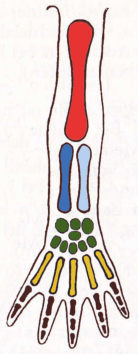
\includegraphics[height=0.35\textheight]{graphics/GrundbauplanExtremitaet_bearbeitet.pdf}} \label{grundbauplan}
  \qquad
  \subfloat[Beispiele]{\includegraphics[height=0.35\textheight]{graphics/ExtremitaetenBeispiele2.pdf}} \label{bsp_extremitaeten}
  
  \caption{Extremitäten von Tetrapoden, Oberarm rot, Speiche dunkelblau, Elle hellblau, Handwurzelknochen grün, Mittelhandknochen gelb, Finderknochen braun\\
  (a) Grundbauplan \cite[S.\ 487, vereinfacht und eingefärbt]{AllgemeineZoologie},\\
  (b) Beispiele für Vordergliedmaßen von Mensch (1), Eidechse (2), Wal (3), Maulwurf (4), Pinguin (5), Pferd (6), Flugsaurier (7), Vogel (8) und Fledermaus (9). \mbox{\cite[S.\ 474]{dtvBiologie}}}
  \label{extremities}
 \end{figure}

% Extremitätengürtel
Schulter- und Beckengürtel bestehen  jeweils aus mehreren Knochen, die je nach Art mehr oder weniger ausgebildet, unterschiedlich geformt oder sogar komplett zurückgebildet sein können \cite[Absatz 9.7]{Vergleichende_Anatomie}. Um das im Folgenden zu vereinfachen, wird jeder Extremitätengürtel durch einen Knochen repräsentiert. Der Schultergürtel wird durch ein Schulterblatt ersetzt und der Beckengürtel durch einen "`Beckenknochen"'.

% verallgemeinerter und abstrahierter Bauplan
\paragraph{Abstraktion}
Das Skelett von Wirbeltieren ist im Allgemeinen also ein kompliziertes Konstrukt aus vielen Einzelteilen, die zwischen verschiedenen Arten stark variieren. Um einen Algorithmus zu entwerfen, der Skeletten nachempfundene Gebilde konstruiert, ist es also notwendig ein erheblich vereinfachtes Modell zu erstellen.\\ 
In Abbildung \ref{bauplan_skelett} ist ein verallgemeinerter und abstrahierter Bauplan für Wirbeltiere zu sehen. Er ist reduziert auf die Wirbelsäule, Rippen, Schädel, Extremitäten, Schulterblatt und Beckenknochen. Die Extremitäten bestehen jeweils aus Oberarm/-schenkel, Unterarm/-schenkel und Hand/Fuß. Hände und Füße werden hier jeweils als ein "`Knochen"' betrachtet, obwohl sie natürlich aus vielen Einzelteilen bestehen. Es kann maximal zwei Extremitätenpaare geben, jeweils einer an jedem Extremitätengürtel. Rippen, Hals- und Schwanzwirbelsäule sind optional und auch die Anzahl der Wirbel und Rippen variiert je nach Tier.

\begin{figure}
 \centering
 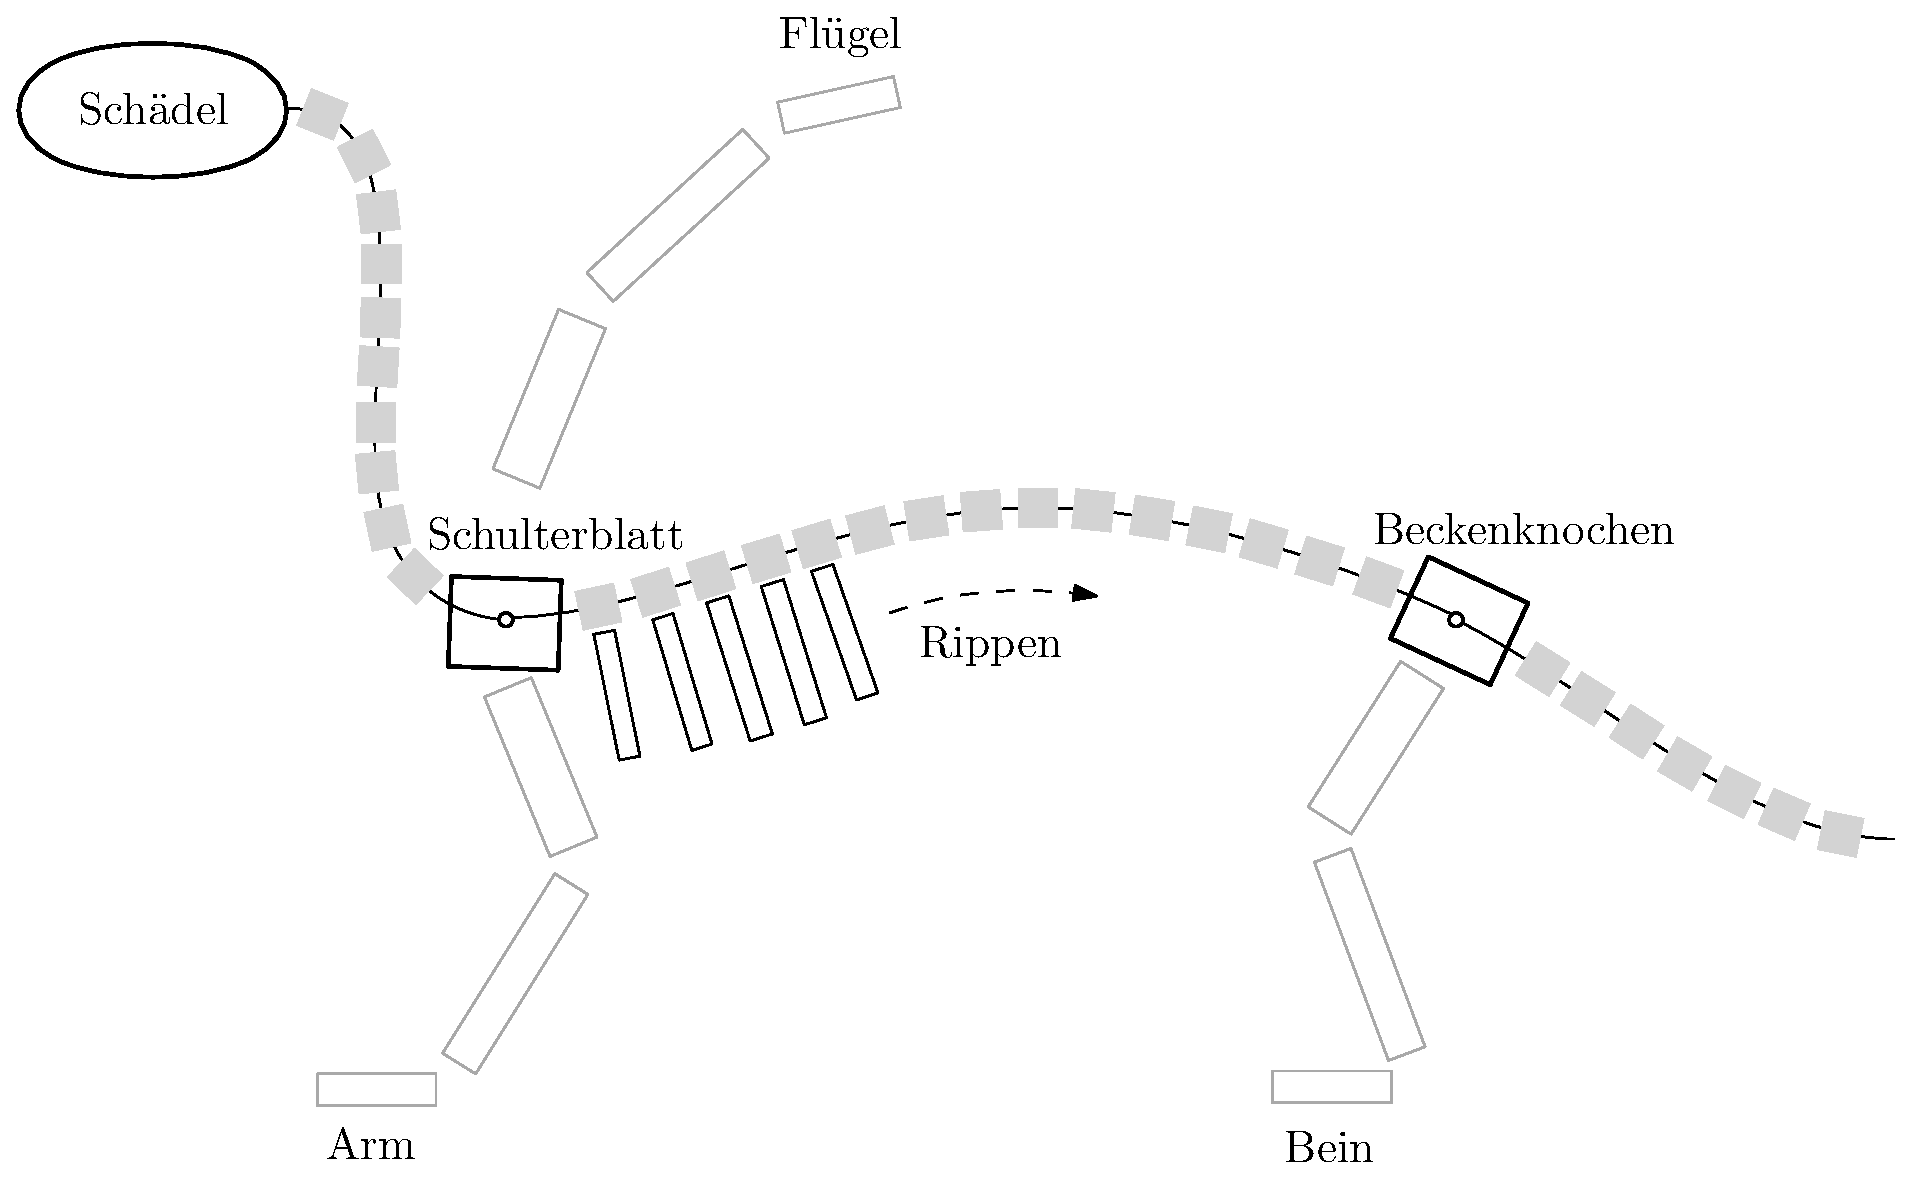
\includegraphics[width=\textwidth]{graphics/skeletonPlan}
 \caption{Verallgemeinerter und abstrahierter Bauplan eines Wirbeltierskeletts. Es sind maximal zwei Extremitätenpaare erlaubt, jeweils eines an jedem Extremitätengürtel. Rippen und Hals- und Schwanzwirbelsäule sind optional. Die Anzahl der Wirbel und Rippen variiert je nach Tier. Oben rechts im Eck ist die Orientierung der Koordinatenachsen angegben.}
 \label{bauplan_skelett}
\end{figure}


%-----------------------------------------------------
\section{Von Groß und Klein}
\label{bigAndSmall}

Dieser Abschnitt widmet sich der Frage nach Unterschieden und Gemeinsamkeiten von großen und kleinen Wirbeltieren. Kann man Wirbeltiere und ihre Skelette einfach vergrößern und verkleinern? Oder sind sie besonders an ihre Größe angepasst? Unterscheidet sich das Skelett einer Maus wesentlich von dem eines Elefanten?

% Extrema
Zunächst ein kurzer Überblick über die Dimensionen, in denen man sich hier bewegt:\\
Das größte und schwerste Wirbeltier ist der Blauwal, er kann bis zu $120$ Tonnen wiegen (siehe \ref{appendix_pca_weight}). Das aktuell kleinste bekannte Wirbeltier, mit einer Länge von $7$ bis $8$mm, ist der Frosch \emph{Paedophryne amauensis} \cite{smallestVertebrate}. Größe und Gewicht von Wirbeltieren kann also erheblich variieren.

% Probleme bei Skalierung
Wenn eine Tierart im Laufe der Evolution wächst, so ändert sich die Größe gleichmäßig. Dieses Wachstum ist aber begrenzt. Der Grund dafür ist, dass die Oberfläche nicht proportional mit dem Volumen mitwächst. Beispielsweise produziert ein Säugetier Wärme proportional zu seinem Volumen. Es kann aber nur Wärme proportional zu seiner Oberfläche abgeben. Dadurch haben große Säugetiere eher Probleme Wärme abzugeben und kleine warm zu bleiben.
Ein ähnliches Problem tritt bei Knochen auf. Die Last, die ein Knochen tragen kann, ist ungefähr proportional zu seiner Querschnittsfläche. Das Skelett muss aber das komplette Gewicht des Körpers tragen, was wiederum proportional zum Volumen ist.
% Lösungen für Skalierungen
Aus diesem Grund müssten die Knochen großer Tiere eigentlich überproportional vergrößert sein. Das ist jedoch nicht unbedingt der Fall. Das Problem an dicken Knochen ist, dass sie den Bewegungsradius, \zb der Extremitäten, stark einschränken. Deshalb passen viele Tiere stattdessen ihre Körperhaltung und Aktivität an, um Spitzenkräfte, wie Stöße oder Oszillationen, auf ihre Knochen zu vermeiden. Deshalb wirken große Tiere auch eher "`behäbiger"' als kleine. \cite[Kapitel 23]{Vergleichende_Anatomie}

Sehr große und sehr kleine Wirbeltiere können also nicht über einfaches Skalieren ineinander überführt werden. Dennoch ähneln sich ihre Skelette sehr.


%-------------------
\section{Mythologie}
\label{biology_mythology}

In diesem Abschnitt wird ein kurzer Blick über die Biologie hinaus, auf fantastische Tiere aus der Mythologie geworfen. 
Ein Algorithmus, der wirbeltierähnliche Skelette erzeugt, bewegt sich ja schon über die Grenzen der Biologie hinaus. Da ist es nur ein kleiner Schritt auch fiktive Wirbeltiere mit zusätzlichen Gliedmaßen zu erzeugen.
Einen guten Überblick über solche Tiere, nicht nur aus der Mythologie sondern auch aus aktuellerer Literatur, Filmen oder Spielen, gibt die Webseite \cite{vertebrateExtraLimbs}.

Hier sollen drei Beispiele hervorgehoben werden, die jeweils charakteristische Merkmale besitzen. Sie stammen aus der Mythologie und bilden oft auch die Grundlage für andere fiktive Wirbeltiere.

\emph{Zentauren} haben einen Pferdekörper, aber statt eines Halses setzt ein menschlicher Oberkörper auf dem Schultergürtel auf \cite{centaurs}. Sie haben also zwei Schultergürtel. 
%\todo{Paper zu Mischwesen zitieren?}

Der \emph{Pegasus} hat ebenfalls den Körper eines Pferdes, aber auch Flügel, die zusätzlich zu den Vorderbeinen am Schultergürtel ansetzen \cite{pegasus}. Es ist also "`möglich"' an einem Extremitätengürtel zwei Paare von Extremitäten ansetzen zu lassen.

\emph{Asiatische Drachen} haben einen langen, schlangenartigen Körper mit oft mehr als vier Beinen. Sie können als Inspiration für Tiere dienen, die mehr als nur zwei Extreimtätengürtel entlang des Rückens besitzen.

